\documentclass[preprint,review,10pt,authoryear,letterpaper]{elsarticle} 
\usepackage{todonotes} 
\usepackage{graphicx}
\usepackage[subrefformat=parens,labelformat=parens]{subfig}
\usepackage{amsmath,url}
\usepackage{amssymb}
\usepackage{booktabs} % Nicer tables
\usepackage{multirow} % Table cells spanning multiple rows
%\usepackage{lineno}
\usepackage[latin1]{inputenc}
\usepackage{tikz}
\usepackage[noperiod]{jabbrv}
\usepackage{listings}


\lstset{
basicstyle=\small\small\ttfamily,
frame=single,	        % adds a frame around the code
breaklines=true,		% sets automatic line breaking
breakatwhitespace=tru,	% sets if automatic breaks should only happen at whitespace
}
\newcommand{\code}[1]{ 
\begin{lstlisting}
#1
\end{lstlisting}
}


\usetikzlibrary{shapes,arrows}
\newcommand{\type}[1]{ {\small\small\tt #1} }
%\usepackage[noperiod]{jabbrv}

\biboptions{comma,sort&compress}

\biboptions{,comma,sort&compress}

\journal{Neuroscience Methods (TBD)}
  
\begin{document}

\begin{frontmatter}

\title{NeuroField: A Neural Field Theory simulation toolbox}


\author{P.K. Fung\corref{ffung}}
\ead{ffung@physics.usyd.edu.au}
\author{R.G. Abeysuriya\corref{}}
\author{X. Zhao\corref{}}
\author{P. M. Drysdale\corref{}}

\author{P.A. Robinson\corref{}}

\address{School of Physics, University of Sydney, New South Wales, Australia}
\cortext[ffung]{Corresponding author. Tel. +61 9036 7274}


\begin{abstract}

Neural field theories are powerful, computationally efficient approach to modeling large-scale brain phenomena. In particular, the versatile neural field theory of Robinson et. al. addresses questions on brain physiology and matches them with experimental observables including the EEG spectra, evoked response potentials, age-related changes to the physiology of the brain, seizures, and synaptic plasticity phenomena. This paper presents NeuroField as a user-friendly, extensible, portable, well-documented software package applicable to simulate a wide range of neural field phenomena, packaged with MATLAB and Python routines for higher-level analysis. NeuroField is %open-source and 
available for non-commercial use at \url{http://physics.usyd.edu.au/brain/neurofield}%under the GNU license 
. 
\end{abstract}

\begin{keyword}
%% keywords here, in the form: keyword \sep keyword
EEG \sep neurophysiology \sep methods \sep modeling
%% MSC codes here, in the form: \MSC code \sep code
%% or \MSC[2008] code \sep code (2000 is the default)

\end{keyword}

\end{frontmatter}

%\linenumbers

\section{Introduction}
\label{sec:introduction}

Neural field theory modeling is a powerful technique for constructing relatively simple, physiologically based models of the brain that are capable of predicting EEG and correlate well with experimental data \cite{Deco2008,Pinotsis2012}. In particular, the neural field theory of Robinson et. al. is a well established theory that addresses the EEG spectra, evoked response potentials, age-related changes to the physiology of the brain, seizures, and synaptic plasticity phenomena \citep{Robinson2005,Rowe2004413,PhysRevE.63.021903,PhysRevE.65.041924,Robinson:04aa,PhysRevE.68.021922,PhysRevE.70.011911,VanAlbada2010,Rennie2002,ker11,Breakspear2006}. In this neural field theory, we make a continuum approximation in which neural properties are averaged over spatial scales of an mm or so: sufficient to contain large numbers of neurons, but small enough to resolve fine structures in brain activities. Within this mean field context, rather than looking at individual neurons, we classify neural populations by the type of neuron (e.g. pyramidal excitatory neurons or inhibitory interneurons), and mean field quantities are label by their spatial position. In each modeling task, we specify the neural populations, stimulations, and synapto-dendritic connections between them (self-connection within a population is allowed), so that each neural population receives local dendritic voltage input and influences other populations via its action potential firing, measured via its instantaneous axonal action potential firing rate. Figure~\ref{fig:ct_schematic} is an example of such a ``population model," where we have two cortical populations and two thalamic populations, with intracortical, intrathalamic, and corticothalamic connections; details about this particular population model can be found in Sec.~\ref{sec:ct}.

\begin{figure}[ht]
\begin{center}
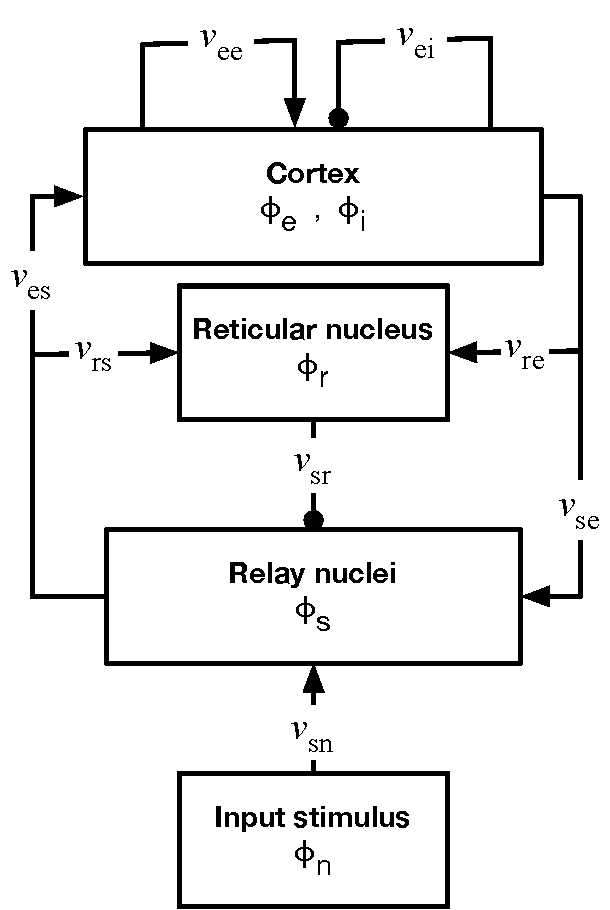
\includegraphics[width=0.50\columnwidth]{EIRS_clean}
\caption{Schematic illustration of the corticothalamic model, which contain excitatory and inhibitory cortical populations (\(e\) and \(i\), respectively), and reticular and relay thalamic populations (\(r\) and \(s\), respectively), where the relay population receives subthalamic stimulation. Arrows indicate excitatory connections, while roundheaded arrows indicate inhibitory connections. This population model is capable of capturing the alpha rhythm, age-related changes to the physiology of the brain, evoked response potentials, seizures, and many other phenomena, as elaborated in Sec.~\ref{sec:ct}.}
\label{fig:ct_schematic}
\end{center}
\end{figure}

The standard theory \citep{Robinson2005} is represented by three equations, which are schematically illustrated in Fig.~\ref{fig:eirs_cycle}.:
\begin{align}
	D_{ab}V_{ab}(\mathbf{r},t) &= \nu_{ab}\phi_{ab}(\mathbf{r},t),\\
			Q_a(\mathbf{r},t) &= S_a \big[\sum_b V_{ab}(\mathbf{r},t) \big],\\
	\mathcal{D}_{ab}\phi_{ab}(\mathbf{r},t) &= Q_b(\mathbf{r},t-\tau_{ab}).
\end{align}
whre the operators \(D_{ab}\), \(S_{a}\), and \(\mathcal{D}_{ab}\) capture synapto-dendritic smoothing, soma response, and axonal propagation of action potentials, respectively, given by

\begin{align}
	D_\alpha(t) &= \frac{1}{\alpha\beta}\frac{d^2}{dt^2} + \left( \frac{1}{\alpha} + \frac{1}{\beta}\right) \frac{d}{dt}+1,\\
	S(V_a) &= \frac{Q_{\textrm{max}}}{1+\exp[-(V_a - \theta)/\sigma']},\\
	\mathcal{D}_a(\mathbf{r},t) &= \frac{1}{\gamma_a^2}\frac{\partial^2}{\partial t^2} + \frac{2}{\gamma_a}\frac{\partial}{\partial t} + 1 - r_a^2\nabla^2,
\end{align}

In these equations, all dynamical quantities and operations are subscripted with population indices \(a\) (if it is associated with population \(a\)) or \(ab\) (if it is associated with the connection from \(b\) to \(a\)). The mathematical symbol \(\phi\) represents the axonal firing rate, \(\nu\) represents local somato-dendritic coupling strength, \(V_{ab}\) denotes the connection \(ab\)'s contribution to the soma voltage potential, which is summed via \(\sum_b V_{ab}\) to give the population soma voltage potential \(V_a\); \(Q\) is the population firing rate, which feeds into the axonal firing rate with a time delay \(\tau\). All neural quantities carry spatial and temporal dependencies. The operator parameters \(\alpha\) and \(\beta\) are the rise and decay rates of dendritic response, \(Q_\textrm{max}\) is the maximum firing rate, \(\theta\) is the mean firing threshold, \(\sigma'\) is the population standard deviation of the soma voltage relative to threshold, \(\gamma\) is the temporal damping coefficient, and \(r\) is the spatial effective range of axonal propagation. This can be schematically summarized in Fig.~\ref{fig:eirs_cycle}.

\begin{figure}[ht]
\begin{center}
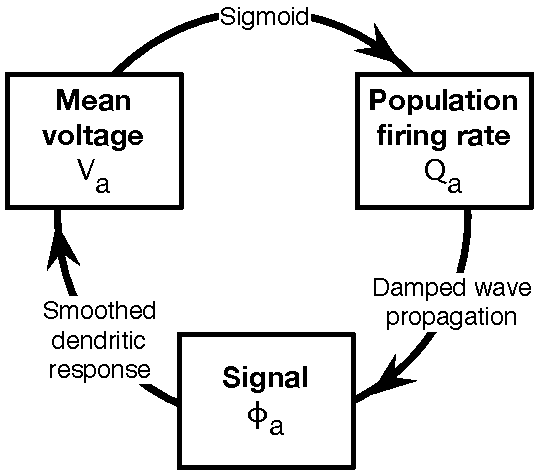
\includegraphics[width=0.40\columnwidth]{EIRS_cycle}
\caption{Schematic overview of the key dynamic quantities \(V_a\), \(Q_a\) \(\phi_{ab}\) in the neural field model, as governed by Eqs~(1)--(3).}
\label{fig:eirs_cycle}
\end{center}
\end{figure}

Of course, one of the major strengths of the neural field theory of \citet{Robinson2005} is its versatility: by choosing the appropriate neural population model, we may model cortical phenomena \citep{}, the corticothalamic system \citep{}, or even hemispheric interactions \citep{}. Moreover, we may replace the operators above with more sophisticated ones, so as to model additional phenomena. For example, by replacing the constant synapto-dendritic coupling strength \(\nu\) with a dynamic one, we may model synaptic plasticity (see Sec.~\ref{sec:cadp}). Or, by replacing the sigmoidal soma firing response with differential equations, we can capture bursting firing rates (see Sec.~\ref{sec:burst}).

This versatility and extensibility of the theory presents a challenge in the implementation of the numerical solver. First, we need a program that takes an arbitrary number of neural populations, with possibly different population types and parameters for each population, and arbitrary connections between the populations, where again each connection may be of different types and is described by different parameter values. Several factors contribute to making the numerical integration of equations difficult: propagation delays between neural populations result in delay-differential equations that require special handling of temporal history; propagation of action potentials according to a damped wave equation adds two spatial dimensions to the system; periodic boundary conditions must be correctly handled during the integration. The popularity and extensibility of the theory means that the program will involve many developers, who extend and reuse previous code independently; coding level structure needs to be in place to ensure proper collaborative effort and minimizing the chance of error.

We have developed NeuroField as a software package that solves the neural field equations for arbitrary neural population models that is user-friendly and easily extensible. Written in C++, this code has been tested on a range of Linux distributions, Microsoft Windows, and Mac OS X. Front-ends written in MATLAB and Python are also provided for analysis and visualization. In this paper, we present the software as a solution to quickly testing and analyzing neural field models. This paper is structured as follows: in Sec.~\ref{sec:method}, we present the usage of NeuroField, including the MATLAB and Python interfaces, as well as the numerical algorithm of NeuroField; in Sec.~\ref{sec:results}, we present example usages of NeuroField in published neural field theory as a showcase of the capabilities of NeuroField. Separate manuals that provide documentations to all user options, extension procedures and coding algorithms are bundled with the NeuroField package.

\section{Method}
\label{sec:method}

We present NeuroField, a C++ program bundled with MATLAB and Python scripts as a flexible numerical package specialized in solving Eqs~(1)--(6). The program reads a human readable configuration file (abbreviated as the config file), which specifies all the simulation information, including an arbitrary population model, (i.e., the number of populations and the connections between them,) and the type and parameter values of each population and connection. Given the config file, NeuroField creates a human readable output file, which stores the time series of the neural quantities as requested by the user. Optional MATLAB and Python scripts are packaged with NeuroField to aid the launching and output analysis of the simulation. Figure~\ref{fig:workflow} is a flow diagram summarizing the workflow of NeuroField usage. Ample documentation of all usage options, config file options and scripting interfaces are bundled with the software package, so that we will not exhaust these information in this paper. Below, we first explain the structure and algorithm of the program in Sec.~\ref{sec:neurofield}, and in Sec.~\ref{sec:interface}, we provide a brief overview of the interfaces of NeuroField.

\begin{figure}[th]
\begin{center}
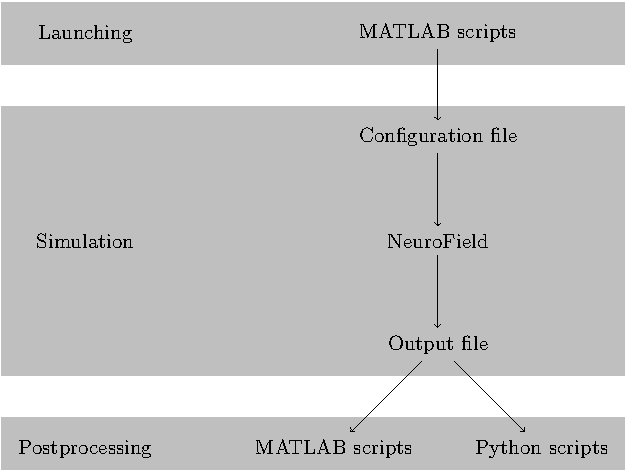
\includegraphics[scale=.8]{flow.pdf}
\caption{Flow diagram illustrating typical NeuroField usage workflow, which can be categorized into three broad phrases: launching, simulation, and postprocessing. The core is the simulation phase, where NeuroField reads the configuration file (or config file for short), and generates the output file, which stores the simulation results. In the postprocessing phase, the simulation results are further analyzed and useful data, plots, figures may be generated. MATLAB and Python routines are provided to aid postprocessing. Similarly, MATLAB and Python wrapper scripts are provided to aid the creating and running of config files. Since both the config file and output file are human readable, they may be processed manually, and the use of any MATLAB and Python scripts are optional. Section~\ref{sec:neurofield} elaborates on the simulation phase, while Sec.~\ref{sec:interface} elaborates on the launching and postprocessing phases. In Sec.~\ref{sec:results} we present illustrative examples of NeuroField simulation results applied onto recent research.}
\label{fig:workflow}
\end{center}
\end{figure}

\subsection{Simulation algorithms}
\label{sec:neurofield}

The NeuroField program uses standard C++ features including object-oriented programming, templates programming, and the C++ standard library, and has been tested on a range of Linux distributions, Microsoft Windows, and Mac OS X.
% history: Peter Drysdale wrote the first version, Felix Fung rewrote the entire code, but all the algorithm is still Peter Drysdale's.

To solve Eqs~(1)--(6), NeuroField creates objects to handle the time integration of neural dynamical quantities. Each population is associated with a firing response to handle Eqs~(2) and (5), while each connection between two populations is associated with the axonal propagation of the instantaneous firing rate of the presynaptic neural population (to handle Eq.~(3) and (6)), and the synaptic and dendritic coupling of the postsynaptic population (to handle Eqs~(1) and (4)). We may rearrange Eqs (1)--(3) into this form to illustrate the division of the system of partial differential equations:
\begin{align}
	P &= \nu_{ab}\phi_{ab}, & \text{Synaptic coupling}\\
	D_{ab}V_{ab} &= P, & \text{Dendritic response}\\
	Q_a &= S_a \big[\sum_b V_{ab} \big], & \text{Firing response}\\
	\mathcal{D}_{ab}\phi_{ab} &= Q_b,&  \text{Axonal propagation}
\end{align}
which can be schematically summarized in Fig.~\ref{fig:components}.

\begin{figure}
\begin{center}
\tikzstyle{pop_style} = [rectangle, draw, text width=6em, text centered, minimum height=4em]
\tikzstyle{couple_style} = [rectangle, draw, text width=6em, text centered, minimum height=4em,fill=gray!30]
\tikzstyle{line} = [draw, -latex']    
\begin{tikzpicture}[node distance = 2.7cm, auto]
	\node[pop_style] (qresponse) {Firing response\\$\sum_bV_{ab} \rightarrow Q_a$};
    %\node[pop_style,right of=qresponse] (pop) {\texttt{Population}\\$Q_b$};
    \node[couple_style,right of=qresponse] (propag) {Axonal propagation\\ $Q_b \rightarrow \phi_{ab}$};
    \node[couple_style,right of=propag] (couple) {Synaptic coupling\\$\phi_{ab} \rightarrow \nu_{ab}\phi_{ab}$};
    \node[couple_style,right of=couple] (dendrite) {Dendritic response\\$\nu_{ab}\phi_{ab}\rightarrow V_{ab}$};
    \draw[line] (qresponse) -- (propag);
    \draw[line] (propag) -- (couple);
    \draw[line] (couple) -- (dendrite);
\end{tikzpicture}
\caption{Flow diagram illustrating the NeuroField algorithm, where each equation of \citet{Robinson2005} is handled by a C++ object. Here, a firing response (white fill) is associated with each neural population, while each gray-filled objects are associated with each connection between two populations. Compare with Fig.~\ref{fig:eirs_cycle}. Importantly, each object may be extended or replaced via C++ inheritance, so that new object types provide extension to the standard \citet{Robinson2005} theory.}
\label{fig:components}
\end{center}
\end{figure}

All numerical integrations involves explicit direct integration, except for Eqs.~(10). Much of the complexity of NeuroField lies in the solving of this delay-partial differential equation with spatial dependence. Correct, efficient implementation of this step tends to be the biggest hurdle to implementing a neural field model. NeuroField solves by storing the neural firing rate  histories and uses explicit finite differences integration. By default, Euclidean geometry with toroidal topology is used. However, non-Euclidean geometry or alternative boundary conditions may be implemented, so that simulation may be performed on surfaces such those found in structural MRI in the future.

Importantly, NeuroField uses the object-oriented feature of C++, so that these classes of objects may be extended or replaced. For example, while in the standard theory of \citet{Robinson2005} the synaptic coupling strength \(\nu_{ab}\) is constant, we may extend the synaptic coupling class via inheritance to implement synaptic plasticity, which will be elaborated in Sec.~\ref{sec:cadp}. Another example is to introduce a non-sigmoidal firing response to introduce burst firing, to be elaborated in Sec.~\ref{sec:burst}. In addition, a generic 4\textsuperscript{th} order Runge-Kutta solver is implemented for all NeuroField objects, and a generic 9-point stencil for numerical integration involving spatial dependency is available. A developer's guideline is bundled with the NeuroField package, which provide a complete document on the algorithm and code structure of NeuroField, as well as guideline for code development. Thus, extension of the neural field theoretic equations is very simple in NeuroField, where the development time may be in the order of only a few hours.

\subsection{User interfaces}
\label{sec:interface}

As shown in Fig.~\ref{fig:workflow}, the core NeuroField C++ program takes in a plain text configuration file (abbreviated as the config file), where the user specifies all the simulation information, and write the simulation result into a output file. A separate user manual, that is bundled with the software package, exhaustively documents all the options for the user interface, so that it will not be repeated here. Rather, we provide a brief overview of the interface below, and Sec.~\ref{sec:results} presents illustrative results.

Table~\ref{tab:task} tabulates typical NeuroField usage tasks, and the corresponding work required. Most tasks involve only editing the config file, and then postprocessing the simulations results, so that only the launching and postprocessing phase in Fig.~\ref{fig:workflow} requires attention. Even so, ample helper scripts exist to aid both the launching and postprocessing phase.

\begin{table}
	\begin{tabular}{ p{4.2cm} p{4.5cm} l }
	\hline
	Task & Action & File \\
	\hline
	Perform simulation & Run NeuroField manually, or via helper scripts & --- \\
	%Visualize/analyze results & --- & MATLAB and Python helper scripts \\
	Parameter exploration & Change parameter value & In config file \\
	Use alternative object type & Change object type & In config file \\
	Use alternative population model & Change connection matrix and objects & In config file \\
	Create new object type & Write new C++ class & In source code \\
	\hline
\end{tabular}
\caption{NeuroField tasks requirements, in roughly ascending order of difficulty, so that a task lower in the table often involve also doing the tasks above the entry. Most simulations require only editing of the config file; only the creation of new object types require code writing. Even for the latter, ample documentation, guidelines and working examples minimizes the coding workload. See also Fig.~\ref{fig:workflow} for NeuroField usage workflow and interface.}
\label{tab:task}
\end{table}

\subsubsection{Input}

Figure~\ref{fig:config_text} is an example config file for the neural field model to be discussed in Sec.~\ref{sec:wave}. The config file starts with a descriptive comment. Then, simulation parameters including simulation duration and time step size, and the number of spatial nodes are specified. This is followed by the specification of a square connection matrix, where a non-zero entry indicate a connection between two populations, so that each connection consists of a axonal propagation from the presynaptic neural population, and a dendritic and firing response from the postsynaptic population. Then, each neural field object, which include firing response ({\tt Firing}), dendritic response ({\tt Dendrite}), axonal propagation ({\tt Propag}) and synaptic coupling ({\tt Couple}), is specified via a {\tt identifier: type - } syntax, followed by the designated parameter values, which follow a {\tt parameter: value} syntax. In the example of Fig.~\ref{fig:config_text}, the axonal propagation of the excitatory-excitatory self-coupling ({\tt Propag 1}) is a ``wave" type propagation, that has a characteristic spatial range of 0.2 m and a damping coefficient of 30 s\textsuperscript{-1}.

\begin{figure}[!htbp]
\begin{center}
\begin{lstlisting}
Example config file for one-population neural field model
Time: 0.15 Deltat: 1e-4
Nodes: 900

Connection matrix:
From:  1  2 
To 1:  1  2  
To 2:  0  0  

Population 1: Excitatory
 Length: 0.5
 Q: 10.98
 Firing: Sigmoid - Theta: 0.013 Sigma: 0.0038 Qmax: 340
  Dendrite 1: alpha: 83 beta: 769
  Dendrite 2: alpha: 83 beta: 769

Population 2: Stimulation
 Length: 0.5
 Stimulus: Pulse - Onset: 0 Node: 465 Amplitude: 1 Width: 1e-3 

Propag 1: Wave - Range: 0.2 gamma: 30
Propag 2:  Map -
Couple 1:  Map - nu: 1e-4
Couple 2:  Map - nu: 1e-4

Output: Node: All Start: 0 Interval: 1e-4
Population: 1
Dendrite:  
Propag: 1
Couple:  
\end{lstlisting}
\caption{Example config file, for a one-population model receiving a pulse stimulus. Details and result of this system can be found in Sec.~\ref{sec:wave}.}
\label{fig:config_text}
\end{center}
\end{figure}

\begin{figure}[th]
\begin{center}
\begin{lstlisting}
    Time  |             Pop.1.V  |        Dendrite.1.V  |
          |                   1  |                   1  |
5.00e-03  | -1.020386100923e-03  |  2.589927678839e-02  |
1.00e-02  | -1.020386100890e-03  |  2.589927678842e-02  |
\end{lstlisting}
\caption{Example output file from NeuroField, where the time series of two neural dynamic quantities are outputted in columns. The first line provides the column heading, while the second line provides the spatial node index. Each subsequent line is outputted at a simulation time interval as the user dictated in the config file.}
\label{fig:output_text}
\end{center}
\end{figure}

\subsubsection{Output}

The outputting of simulation results are specified in the end of the config file. In Fig.~\ref{fig:config_text}, the excitatory population and the excitatory-excitatory axonal propagation is specified to be outputted, so that these two objects will output the time series of their neural dynamical quantities, which in this case will be population soma voltage and axonal firing rate, respectively. To ensure numerical stability, the equations need to be integrated with a very small time step (e.g., $1\times10^{-4}$\,s$=10000$\,Hz). This is much smaller than typically required for analysis; EEG is typically sampled at just 500~Hz or less. To reduce output file size and avoid unnecessarily long postprocessing computation, an output sampling interval can be specified, downsampling the output from NeuroField.

Figure~\ref{fig:output_text} shows an example output file; given it is human readable, standard tools may be used to analyze these data, in addition to the provided MATLAB and Python scripts. In Sec.~\ref{sec:postprocess-manual}, we explain that users can manually edit the human-readable interfaces to use NeuroField, and in Sec.~\ref{sec:postprocess-matlab}, we provide an overview on the MATLAB helper scripts that is bundled with NeuroField as additional interface.

\subsubsection{Manual read/write}
\label{sec:postprocess-manual}

Given that both the config file and output file are human readable (see Fig.~\ref{fig:config_text} and Fig.~\ref{fig:output_text}), manual usage of NeuroField without any helper scripts is possible, by writing the config file and reading the output file. This is particularly true as ample documentation and working example config files exist. Indeed, one convenient way of starting a simulation involves editing an existing config file until it matches the intended simulation environment, and running NeuroField. Since the output file is plain-text, it is very easy to use standard tools to perform postprocessing analysis on the simulation results. For example, a simple PERL script that calls gnuplot exists for simple time series plotting.

\subsubsection{MATLAB helper scripts}
\label{sec:postprocess-matlab}

In addition to manually editing the plain-text files, NeuroField is packaged with MATLAB helper scripts that assists with both the launching of NeuroField and postprocessing of simulation results.

The usage of these MATLAB scripts involves first reading the simulated results from the NeuroField output file into an ``NF" MATLAB object, via an {\tt nf\_read()} function, and then using the {\tt nf\_extract()} function to extract neural dynamic quantities. Then, numerous scripts are provided for visualization, including plotting routines and animation routines, and also routines for the calculation of power spectra. In Sec.~\ref{sec:results}, we provide numerous examples of NeuroField simulations results, where the generation of these figures rely heavily on these helper scripts.

\todo[inline]{More from Romesh}

\begin{figure}[th]
\begin{center}
\begin{lstlisting}
function nf_example_plot(fname)
  % read simulation result into NF object
  NF = nf_read( [fname,'.output'] );
  % extract simulation time points
  time = nf.time;
  % extract population voltage
  v = nf_extract( nf, 'Pop.1.V' );
  % plot the result
  plot( time, phi );
\end{lstlisting}
\caption{Example MATLAB postprocessing, utilizing the {\tt nf\_read()} and {\tt nf\_extract()} functions provided by NeuroField to plot simulation data. In addition to 2D plotting, other functions including animation and spectral plots are also included.}
\label{fig:matlab_eg}
\end{center}
\end{figure}

%There are a number of common ways to analyze the output from neural field models. First, plots of the time series are useful for directly viewing neural oscillations, evoked responses, seizures, monitoring plasticiity, and verifying stability. Second, calculation of the power spectrum, which is often compared to experimental EEG. This can also involve detection of multiple spatial modes of activity and incorporation of volume conduction, to account for effects introduced by electrodes in real-world recordings. Finally, spatial patterns of activity and propagation of waves of activity can be visualized on a surface plot. All of these basic analyses are included as Matlab programs in the NeuroField toolbox. 
%
%The nf\_extract() function makes it easy to select data for plotting from a NeuroField object. nf\_movie can plot an animation of the output
%
%NeuroField is packaged with several helper scripts written in MATLAB to assist with running, analyzing and visualizing models. 
%
%nf\_read() allows users to parse the output file from NeuroField into a MATLAB struct object.
%nf\_grid reshapes the output for handling matrices. 
%
%nf\_eirs() demonstrates writing a configuration file, running it with nf\_run(), and then reading it with nf\_read(). This demonstrates a complete MATLAB-based toolchain for using NeuroField.
%

\todo[inline]{Python scripts? John Griffiths}

\section{Results}
\label{sec:results}

In this section, we present examples of NeuroField simulation results applied to recent research as a showcase of the capabilities of NeuroField. All plots and figures are simulation results of NeuroField, where the plots are generated by the helper scripts explained in Sec.~\ref{sec:postprocess-matlab}.

\subsection{Single excitatory population model}
\label{sec:wave}

\begin{figure}[t]
\begin{center}
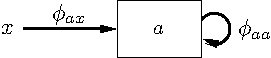
\includegraphics[width=0.50\columnwidth]{one-pop}
\caption{Schematic diagram of a single excitatory population model, which feeds back to itself and receive an external stimulus. This constitutes the simplest neural field model that conforms to Eqs~(1)--(6).}
\label{fig:ct_schematic}
\end{center}
\end{figure}

We first present the simplest neural field model possible, consisting of a single excitatory population that feeds back to itself, and receiving an external stimulus. All neural dynamics are as Eqs~(1)--(6), so that this model conforms to the standard \citet{Robinson2005} theory. The config file is shown in Fig.~\ref{fig:config_text}, and no extension of NeuroField coding is required. All parameters are taken from \citet{Robinson:04aa}, with the exception of the axonal propagation parameters, which are tuned to emphasize wave propagation properties for illustrative purposes.

Figure~\ref{fig:wave_comparison} presents the neural dynamics of the system in two snapshots, as generated by the MATLAB helper scripts presented in Sec.~\ref{sec:postprocess-matlab}. Here, the \(x\) and \(y\) coordinates are spatial coordinates, and the vertical axis plots the axonal firing rate as a measure of neural activity. Figure~\ref{fig:wave_comparison}~(a) show that the neural dynamics of the population is in a steady state and has achieved spatial homogeneity, while receiving a stimulus in the middle. Figure~\ref{fig:wave_comparison}~(b) shows the neural dynamics at a later time instance, and we see that the stimulus spread according to damped wave propagation. In addition to generating plots, one MATLAB helper script (see Sec.~\ref{sec:postprocess-matlab}) also generates movies, which would aid the analysis of wave propagation in this example.

\todo[inline]{Romesh please check transient vs stable state and stimulation onset (and why are we plotting V and phi?)}

\begin{figure}[t]
\begin{center}
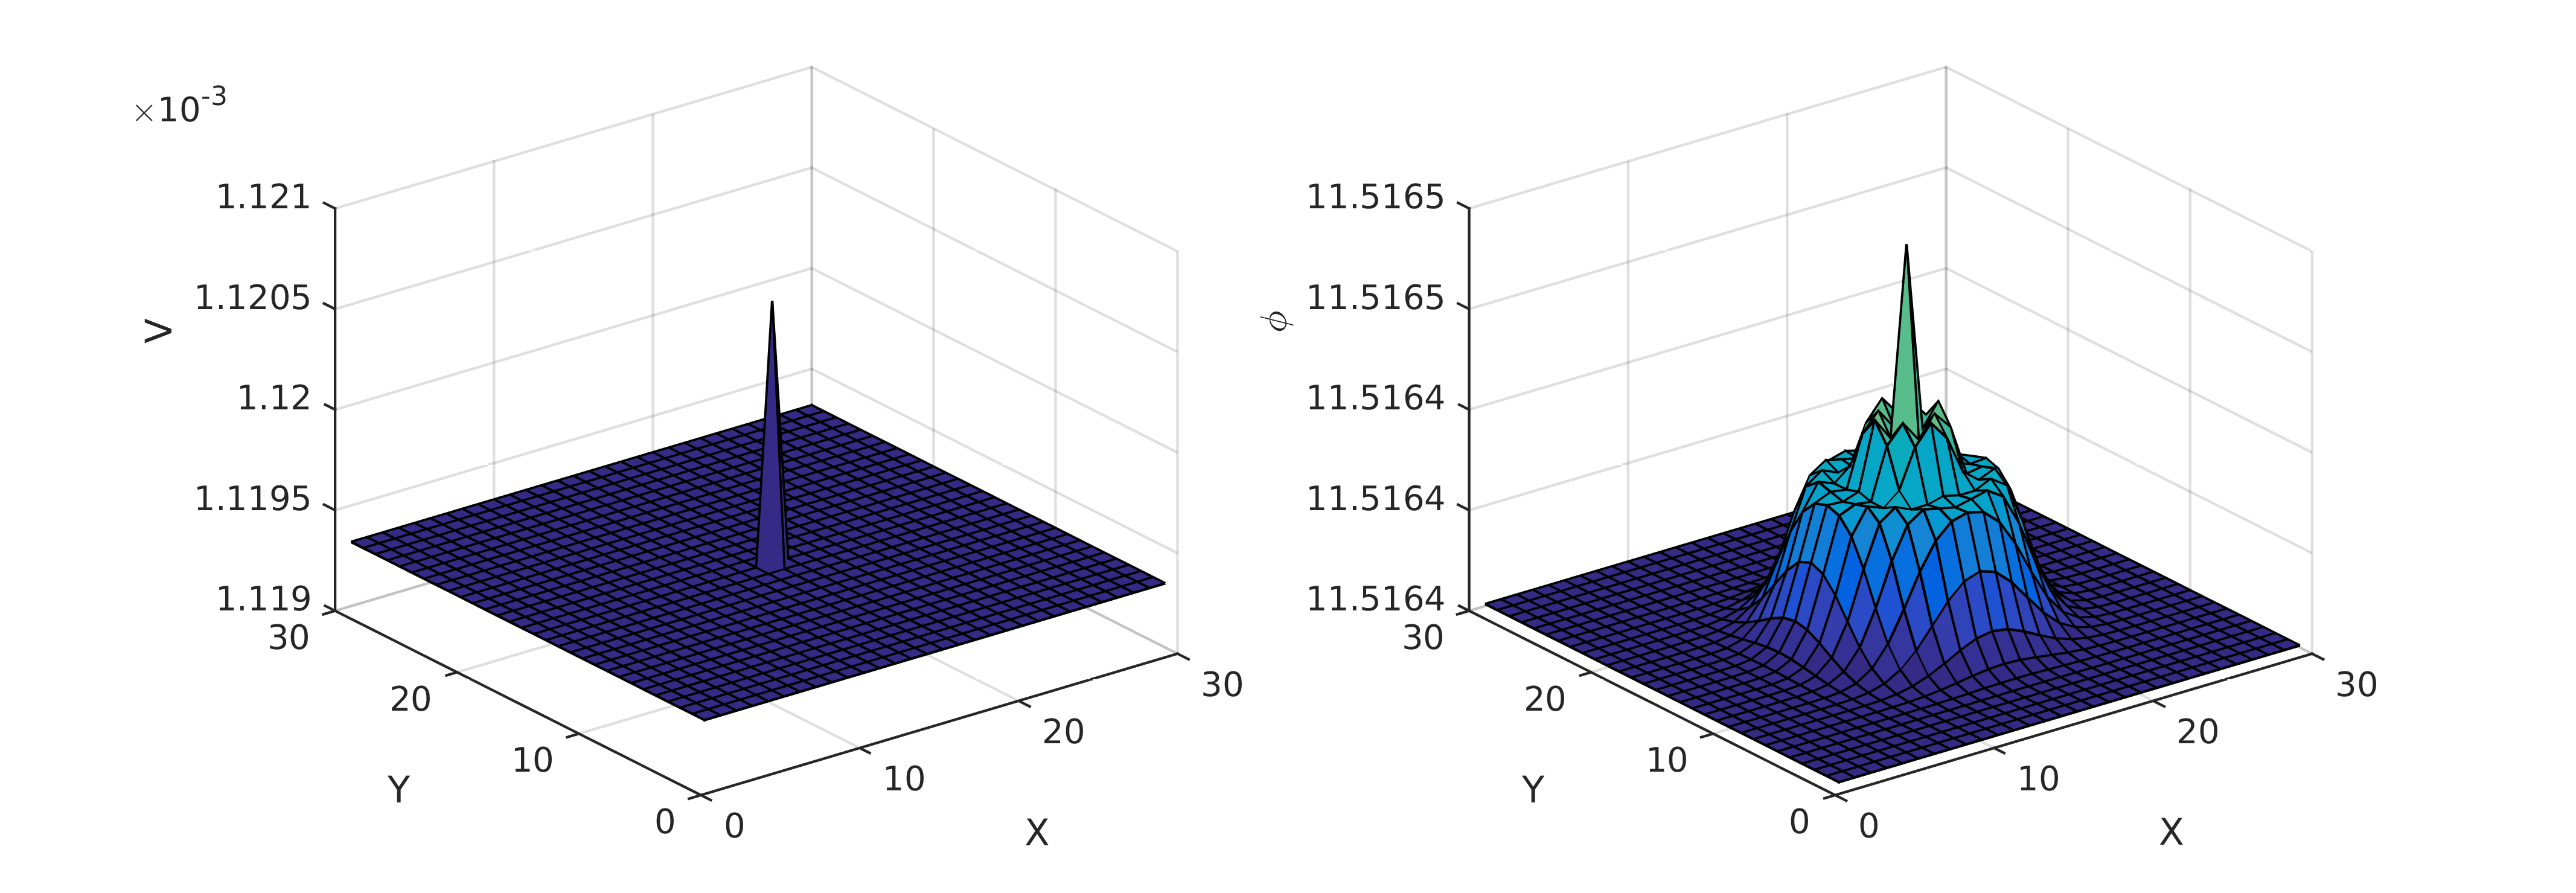
\includegraphics[width=.9\textwidth]{wave_comparison}
\caption{Two plots on the neural activity of the one-population model first introduced in Fig.~\ref{fig:one-pop}. The \(x\) and \(y\) coordinates are spatial coordinates, while the vertical axis is the axonal firing rate, which serves as a measure of neural activity. (a) Neural activity is in a steady state, where the firing rate is spatially homogeneous, while receiving a stimulus in the middle. (b) Neural activity propagates radially outwards, as governed by the damped wave equation~(6).}
\label{fig:wave_comparison}
\end{center}
\end{figure}

\todo[inline]{Put labels (a) and (b) into figure.}

\subsection{Single population with synaptic plasticity}
\label{sec:cadp}

The single-excitatory population model of Sec.~\ref{sec:wave} may be extended to model synaptic plasticity. \citet{fung13} and \citet{fung14} extended the standard theory of \citet{Robinson2005} by introducing time dependence on the synapto-dendritic coupling strength \(\nu\) in Eq.~(7), to model the experimental results found in transcranial magnetic stimulation (TMS). The coding implementation is done by inheriting the synaptic coupling class, and using the generic 4\textsuperscript{th} order Runge-Kutta solver provided in NeuroField.

Figure~\ref{fig:cadp} shows a schematic diagram for the synaptic plasticity theory of \citet{fung13} and \citet{fung14}, illustrating how neural activity leads to intraneuronal calcium influx, which signals synaptic plasticity expression, which in turn is modulated by metaplasticity on a longer timescale. Figure~\ref{fig:cadp-window} presents a comparison between experimental results and NeuroField simulation results in paired associative stimulation (PAS), a variation of TMS experiment. The reproduction of experimental result via the introduction of mean field calcium level and synaptic plasticity into neural field theory demonstrates the flexibility and extensibility of NeuroField.

\begin{figure}[t]
\begin{center}
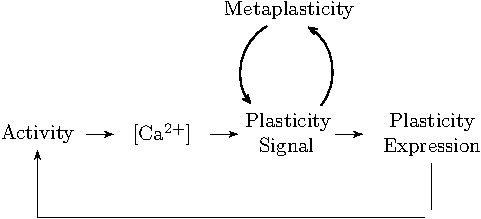
\includegraphics[width=.7\textwidth]{bcm-schematic}
\caption{Schematic diagram illustrating the plasticity theory used in \citet{fung13} and \citet{fung14}. Within the context of neural field theory, we introduce mean field intraneuronal calcium and non-static synaptic coupling strength, so that neural activity leads to intraneuronal calcium influx, which signals synaptic plasticity, which in turn is modulated by metaplasticity. Expression of synaptic plasticity feeds back into neural activity, introducing a loop. This is implemented into NeuroField via C++ inheritance on the synaptic coupling object, and using the generic 4\textsuperscript{th} order Runge-Kutta solver provided. Figure reproduced from \citet{fung14}.}
\label{fig:cadp}
\end{center}
\end{figure}

\begin{figure}[t]
\begin{center}
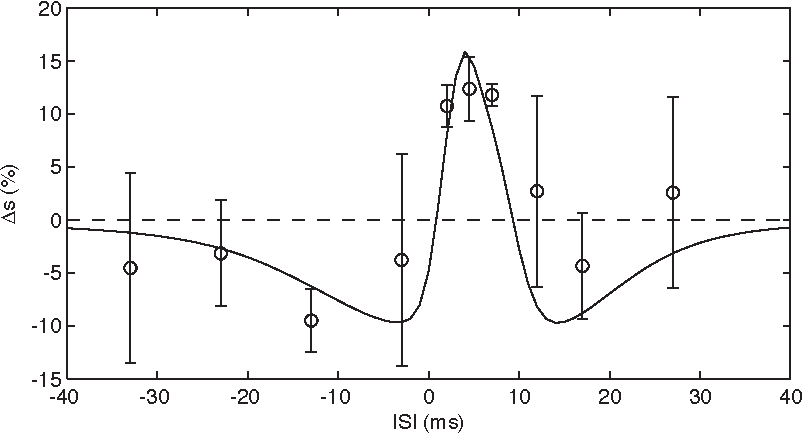
\includegraphics[width=.8\textwidth]{window}
\caption{Experimental and simulation results of paired associative stimulation (PAS), where transcranial magnetic stimulation and peripheral electric stimulation is applied with an inter-stimulus interval (ISI) in between. Depending on the size and ordering of the ISI, different size and direction of synaptic plasticity may be induced. Dots and error bars: mean and standard deviation from experiments; line: NeuroField simulation result. Figure reproduced from \citet{fung13}.}
\label{fig:cadp-window}
\end{center}
\end{figure}

\subsection{Corticothalamic model (Romesh)}
\label{sec:ct}

NeuroField has been extensively tested with a recent neural field corticothalamic model of the brain \citep{Robinson2005,Rowe2004413,PhysRevE.63.021903,PhysRevE.65.041924,Robinson:04aa} that we have previously used to investigate the alpha rhythm \citep{PhysRevE.68.021922,PhysRevE.70.011911}, age-related changes to the physiology of the brain \citep{VanAlbada2010}, evoked response potentials \citep{Rennie2002,ker11}, seizures \citep{Breakspear2006}, and many other phenomena. 

The structure of the model is shown in Fig.~\ref{fig:ct_schematic}. Much of our work is in the linear regime and utilizes analytic results for small perturbations to steady states. In the steady state, we have

We thus obtain the equation for the steady state firing rate equal to $\phi_e^{(0)}$ \cite{Robinson:04aa}
\begin{align}
	\label{eqn:ve_root}
	\begin{split}
	S^{-1}&(\phi_e^{(0)})-(\nu_{ee}+\nu_{ei})\phi_e^{(0)} = \\ &\nu_{es}S\left\{\nu_{se}\phi_e^{(0)}+\nu_{sr}S\left[\nu_{re}\phi_e^{(0)}+(\nu_{rs}/\nu_{es})\left(S^{-1}(\phi_e^{(0)})-(\nu_{ee}+\nu_{ei})\phi_e^{(0)}\right)\right]+\nu_{sn}\phi_n^{(0)}\right\}, 
\end{split}\\[16pt]
	\label{eqn:ve_root_numeric}
	\begin{split}
	V_e^{(0)}&-(\nu_{ee}+\nu_{ei})S(V_e^{(0)})=\\ &\nu_{es}S\left\{\nu_{se}S(V_e^{(0)})+\nu_{sr}S\left[\nu_{re}S(V_e^{(0)})+(\nu_{rs}/\nu_{es})\left(V_e^{(0)}-(\nu_{ee}+\nu_{ei})S(V_e^{(0)})\right)\right]+\nu_{sn}\phi_n^{(0)}\right\},
\end{split}
\end{align}
where \eqref{eqn:ve_root} and \eqref{eqn:ve_root_numeric} are equivalent.

In the linear regime, we have
\begin{align}
Q_a(\mathbf{r},t) = Q_a^{(0)} + S'\left(V_a^{(0)}\right) \left[V_a(\mathbf{r},t)-V_a^{(0)}\right] \\
+ \frac{S''\left(V_a^{(0)}\right)}{2!} \left[V_a(\mathbf{r},t)-V_a^{(0)}\right]^2 \cdots ,
\end{align}

which can be written in terms of a perturbation by relabeling $Q_a-Q_a^{(0)} \rightarrow Q_a $, $V_a-V_a^{(0)} \rightarrow V_a$, yielding

\begin{align}
\label{eqn:q_series}
Q_a(\mathbf{r},t) &= \rho_a^{(1)} V_a(\mathbf{r},t) + \frac{\rho_a^{(2)}}{2} V_a(\mathbf{r},t)^2 \cdots .
\end{align}


where $\rho_a^{(n)} = S^{(n)}\left(V_a^{(0)}\right)$ and $S^{(n)}$ is the $n$th derivative of the sigmoid function at the steady state value of $Q_a$. 

However, some phenomena are strongly nonlinear, and these must be solved by numerical integration. We have used NeuroField to model results relating to seizures \citep{Roberts2008}, visually evoked potentials \citep{Roberts2012a}, and sleep spindles \citep{Abeysuriya2013,Abeysuriya2013a}. 



\begin{align}
\label{eqn:power_sum}
P(\omega) &= \sum_{m = -\infty}^{\infty}\sum_{n = -\infty}^{\infty} \Delta k_x \Delta k_y |T(\mathbf{k},\omega)|^2||\phi_n(\mathbf{k},\omega)|^2F(k)\\
k^2 &=  \left( \frac{2\pi m}{L_x} \right)^2 + \left( \frac{2\pi n}{L_y}\right)^2 
\end{align}
where the size of the two-dimensional rectangular cortex is $L_x \times L_y$. 

\begin{align}
F(k) &= e^{-k^2/k_0^2},
\end{align}


Prediction of the EEG power spectrum involves two additional steps - first, summation over 

\begin{figure}[!b]
\begin{center}
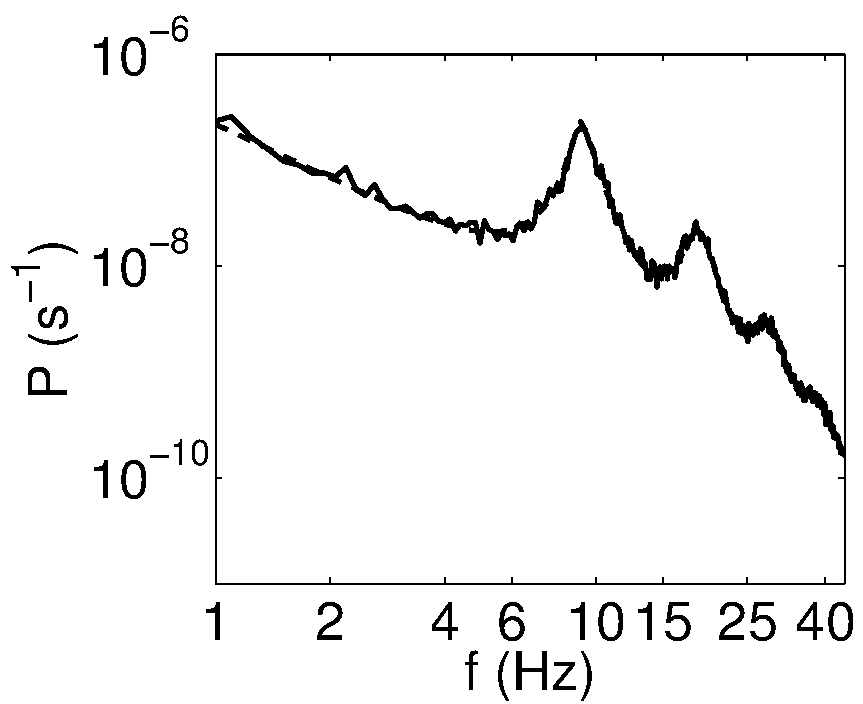
\includegraphics[width=0.80\columnwidth]{corticothalamic_comparison}
\caption{Comparision of linear analytic spectrum with the power spectrum computed using the NeuroField package analysis tools.}
\label{fig:ct_spectrum}
\end{center}
\end{figure}

\begin{figure}[!b]
\begin{center}
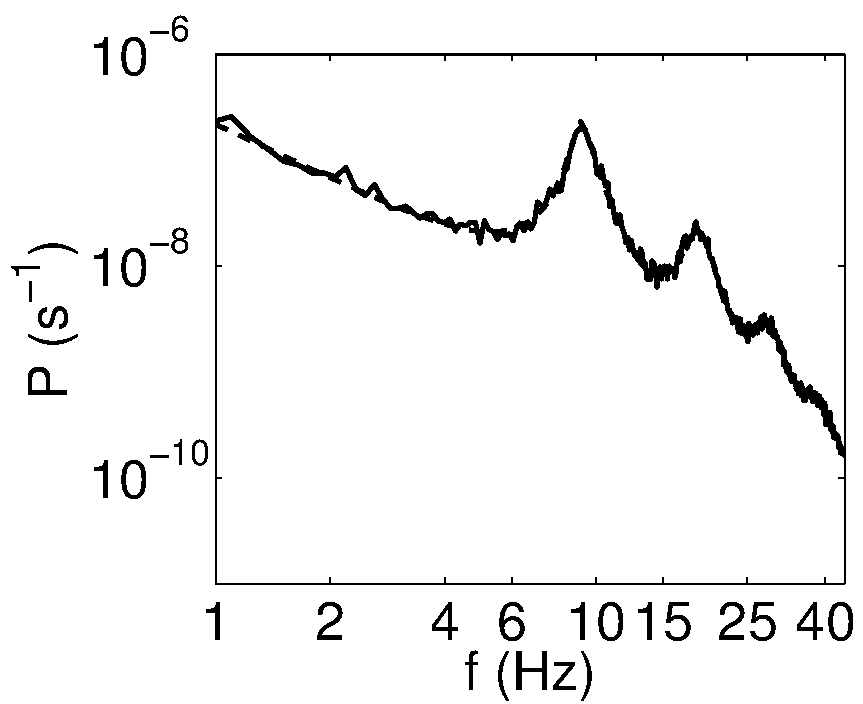
\includegraphics[width=0.80\columnwidth]{corticothalamic_comparison}
\caption{Wake EC, same params as already published}
\label{fig:ct_spectrum_1}
\end{center}
\end{figure}

\begin{itemize}
	\item Sleep spindles
	\item Wake alpha peak
	\item Volume conduction
\end{itemize}

The power spectrum can be obtained by FFT, but correct normalization and calculation of the power spectrum including multiple spatial modes can be challenging to implement. We have implemented a 3D FFT algorithm that correctly normalizes the output and includes volume conduction effects that selective attenuate spatial modes depending on their wavenumber. The result can be directly compared to analytical predictions.

\subsection{Seizures (XL)}
\label{sec:seizures}

\subsection{Corticothalamic model with bursting dynamics (XL)}
\label{sec:burst}

\subsection{Wilson-Cowan model}

\subsection{Jansen-Rit model}

\section{Discussion}
\label{sec:discussion}

We have developed NeuroField to provide an extensible, reliable framework for integrating nonlinear delay differential equations including spatial propagation. NeuroField is aimed for use by researchers who have constructed neural field models of the brain that require numerical integration. In this section, we review some usage and performance considerations.

Most notably, the signals from populations can be associated with local field potentials (LFP) or EEG depending, and these predictions can be directly compared against experimental data. The soma potential or firing rate of the neural populations can be compared to individual neuron data. Changes to synaptic strength can be monitored when simulating neural plasticity. When simulating spatially extended populations, spatial correlations and patterns of activity can also be analyzed. 

\subsection{White noise stimulus}
\begin{itemize}
	\item White noise requires stocastic DE integrator, effectively Euler (FELIX)
	\item Noise amplitude depends on grid resolution as this affects the possible bandwidth. Similar features depend on frequency domain power so noise needs to be normalized correctly (ROMESH)
\end{itemize}

\subsection{Performance}

\begin{itemize}
\item Some numbers about the runtime and memory requirements of NeuroField (FELIX)
\item Note that the memory requirements scale with the grid size, and the grid size depends on Lx and the propagator lengths (automatically enforced) (FELIX)
\item Also that the delays in the system cause O(n) increases in memory usage (FELIX)
\end{itemize}

\todo[inline]{Additional considerations?}

\section{Acknowledgements}
\label{sec:acknowledgements}
This work was supported by the Australian Research Council, National Health and Medical Research Council (through the Center for Integrated Research and Understanding of Sleep), and the Westmead Millennium Institute.

\section{References}
\bibliographystyle{complex_vancouver}
\bibliography{neurofield}

\end{document}

%% References
%%
%% Following citation commands can be used in the body text:
%%
%%  \citet{key}  ==>>  Jones et al. (1990)
%%  \citep{key}  ==>>  (Jones et al., 1990)
%%
%% Multiple citations as normal:
%% \citep{key1,key2}         ==>> (Jones et al., 1990; Smith, 1989)
%%                            or  (Jones et al., 1990, 1991)
%%                            or  (Jones et al., 1990a,b)
%% \citep{key} is the equivalent of \citet{key} in author-year mode
%%
%% Full author lists may be forced with \citet* or \citep*, e.g.
%%   \citep*{key}            ==>> (Jones, Baker, and Williams, 1990)
%%
%% Optional notes as:
%%   \citep[chap. 2]{key}    ==>> (Jones et al., 1990, chap. 2)
%%   \citep[e.g.,][]{key}    ==>> (e.g., Jones et al., 1990)
%%   \citep[see][pg. 34]{key}==>> (see Jones et al., 1990, pg. 34)
%%  (Note: in standard LaTeX, only one note is allowed, after the ref.
%%   Here, one note is like the standard, two make pre- and post-notes.)
%%
%%   \citealt{key}          ==>> Jones et al. 1990
%%   \citealt*{key}         ==>> Jones, Baker, and Williams 1990
%%   \citealp{key}          ==>> Jones et al., 1990
%%   \citealp*{key}         ==>> Jones, Baker, and Williams, 1990
%%
%% Additional citation possibilities
%%   \citeauthor{key}       ==>> Jones et al.
%%   \citeauthor*{key}      ==>> Jones, Baker, and Williams
%%   \citeyear{key}         ==>> 1990
%%   \citeyearpar{key}      ==>> (1990)
%%   \citetext{priv. comm.} ==>> (priv. comm.)
%%   \citenum{key}          ==>> 11 [non-superscripted]
%% Note: full author lists depends on whether the bib style supports them;
%%       if not, the abbreviated list is printed even when full requested.
%%
%% For names like della Robbia at the start of a sentence, use
%%   \Citet{dRob98}         ==>> Della Robbia (1998)
%%   \Citep{dRob98}         ==>> (Della Robbia, 1998)
%%   \Citeauthor{dRob98}    ==>> Della Robbia


%% References with bibTeX database:

%% Authors are advised to submit their bibtex database files. They are
%% requested to list a bibtex style file in the manuscript if they do
%% not want to use elsarticle-harv.bst.

%% References without bibTeX database:

% \begin{thebibliography}{00}

%% \bibitem must have one of the following forms:
%%   \bibitem[Jones et al.(1990)]{key}...
%%   \bibitem[Jones et al.(1990)Jones, Baker, and Williams]{key}...
%%   \bibitem[Jones et al., 1990]{key}...
%%   \bibitem[\protect\citeauthoryear{Jones, Baker, and Williams}{Jones
%%       et al.}{1990}]{key}...
%%   \bibitem[\protect\citeauthoryear{Jones et al.}{1990}]{key}...
%%   \bibitem[\protect\astroncite{Jones et al.}{1990}]{key}...
%%   \bibitem[\protect\citename{Jones et al., }1990]{key}...
%%   \harvarditem[Jones et al.]{Jones, Baker, and Williams}{1990}{key}...
%%

% \bibitem[ ()]{}

% \end{thebibliography}

%%
%% End of file `elsarticle-template-harv.tex'.
